\documentclass{standalone}
\usepackage{amsmath}
\usepackage{tikz}
\usepackage{rotating}
\usetikzlibrary{shapes.geometric, arrows}

\tikzstyle{cat} = [rectangle, rounded corners, 
minimum width=5cm, 
minimum height=1.5cm,
text centered, 
draw=black, 
fill=yellow]

\tikzstyle{typ} = [rectangle, 
minimum width=5cm, 
minimum height=1.5cm, 
text centered,  
draw=black, 
fill=orange!30]

\begin{document}

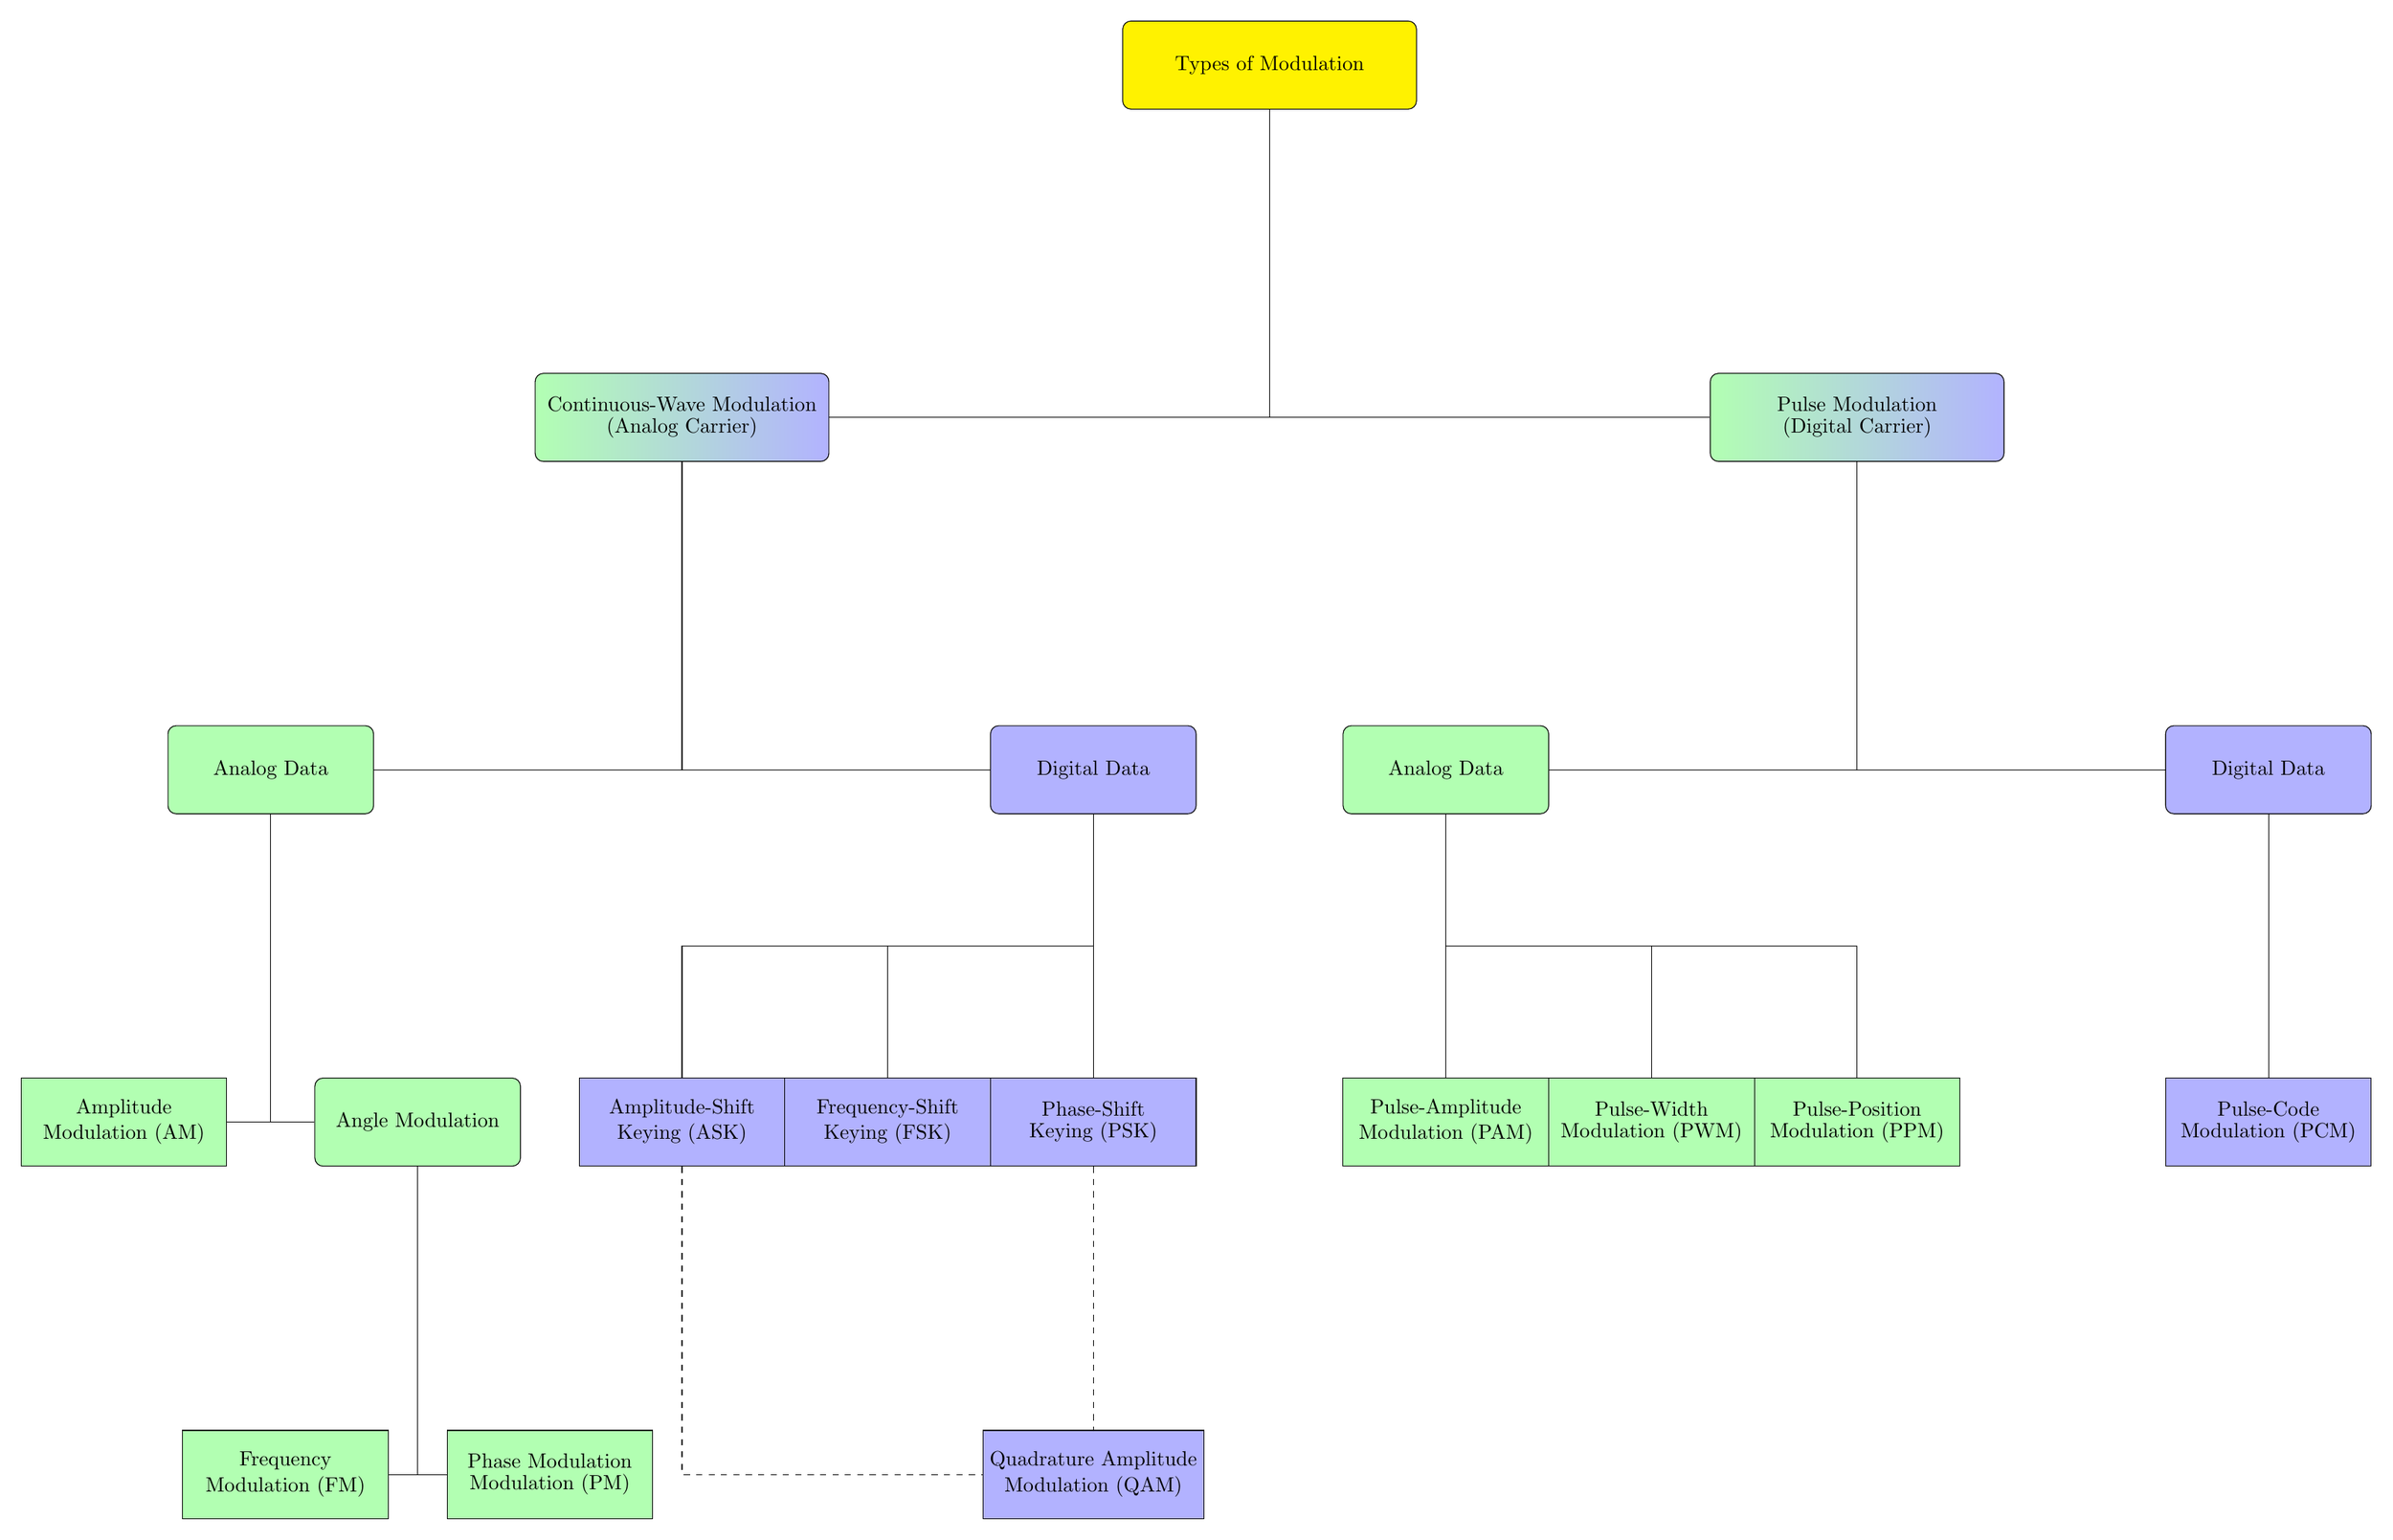
\begin{tikzpicture}[node distance=2cm]

\node (modul) [cat] {Types of Modulation};
\node (cw) [cat, below of=modul, xshift=-10cm, yshift=-4cm, left color=green!30, right color=blue!30] {\shortstack{Continuous-Wave Modulation \\ (Analog Carrier)}};
\node (pulse) [cat, below of=modul, xshift=10cm, yshift=-4cm, left color=green!30, right color=blue!30] {\shortstack{Pulse Modulation \\ (Digital Carrier)}};
\draw[-] (modul) |- (cw);
\draw[-] (modul) |- (pulse);

\node (adat1) [cat, below of=cw, xshift=-7cm, yshift=-4cm, minimum width=3.5cm, fill=green!30] {Analog Data};
\node (ddat1) [cat, below of=cw, xshift=7cm, yshift=-4cm, minimum width=3.5cm, fill=blue!30] {Digital Data};
\draw[-] (cw) |- (adat1);
\draw[-] (cw) |- (ddat1);
\node (adat2) [cat, below of=pulse, xshift=-7cm, yshift=-4cm, minimum width=3.5cm, fill=green!30] {Analog Data};
\node (ddat2) [cat, below of=pulse, xshift=7cm, yshift=-4cm, minimum width=3.5cm, fill=blue!30] {Digital Data};
\draw[-] (pulse) |- (adat2);
\draw[-] (pulse) |- (ddat2);

\node (am) [typ, below of=adat1, xshift=-2.5cm, yshift=-4cm, minimum width=3.5cm, fill=green!30] {\shortstack{Amplitude \\ Modulation (AM)}};
\node (ang) [cat, below of=adat1, xshift=2.5cm, yshift=-4cm, minimum width=3.5cm, fill=green!30] {Angle Modulation};
\draw[-] (adat1) |- (am);
\draw[-] (adat1) |- (ang);
\node (fm) [typ, below of=ang, xshift=-2.25cm, yshift=-4cm, minimum width=3.5cm, fill=green!30] {\shortstack{Frequency \\ Modulation (FM)}};
\node (pm) [typ, below of=ang, xshift=2.25cm, yshift=-4cm, minimum width=3.5cm, fill=green!30] {\shortstack{Phase Modulation \\ Modulation (PM)}};
\draw[-] (ang) |- (fm);
\draw[-] (ang) |- (pm);

\node (ask) [typ, below of=ddat1, xshift=-7cm, yshift=-4cm, minimum width=3.5cm, fill=blue!30] {\shortstack{Amplitude-Shift \\ Keying (ASK)}};
\node (fsk) [typ, below of=ddat1, xshift=-3.5cm, yshift=-4cm, minimum width=3.5cm, fill=blue!30] {\shortstack{Frequency-Shift \\ Keying (FSK)}};
\node (psk) [typ, below of=ddat1, xshift=0cm, yshift=-4cm, minimum width=3.5cm, fill=blue!30] {\shortstack{Phase-Shift \\ Keying (PSK)}};
\node (qam) [typ, below of=psk, xshift=0cm, yshift=-4cm, minimum width=3.5cm, fill=blue!30] {\shortstack{Quadrature Amplitude \\ Modulation (QAM)}};
\draw[-] (ddat1) -- (psk);
\draw[-,dashed] (ask) |- (qam);
\draw[-,dashed] (psk) -- (qam);

\node (pam) [typ, below of=adat2, xshift=0cm, yshift=-4cm, minimum width=3.5cm, fill=green!30] {\shortstack{Pulse-Amplitude \\ Modulation (PAM)}};
\node (pwm) [typ, below of=adat2, xshift=3.5cm, yshift=-4cm, minimum width=3.5cm, fill=green!30] {\shortstack{Pulse-Width \\ Modulation (PWM)}};
\node (ppm) [typ, below of=adat2, xshift=7cm, yshift=-4cm, minimum width=3.5cm, fill=green!30] {\shortstack{Pulse-Position \\ Modulation (PPM)}};
\draw[-] (adat2) -- (pam);

\node (pcm) [typ, below of=ddat2, xshift=0cm, yshift=-4cm, minimum width=3.5cm, fill=blue!30] {\shortstack{Pulse-Code \\ Modulation (PCM)}};
\draw[-] (ddat2) -- (pcm);

\node (node1) [below of=ddat1, xshift=0.125cm, yshift=-1cm] {};
\draw[-] (node1) -| (fsk);
\draw[-] (node1) -| (ask);

\node (node2) [below of=adat2, xshift=-0.125cm, yshift=-1cm] {};
\draw[-] (node2) -| (pwm);
\draw[-] (node2) -| (ppm);

\end{tikzpicture}
\end{document}